\iffalse
\documentclass[10pt,a4paper]{report}
\usepackage[latin1]{inputenc}
\usepackage{amsmath}
\usepackage{amsfonts}
\usepackage{amssymb}
\usepackage{graphicx}
\usepackage{hyperref}
\usepackage{multicol}
\usepackage[margin=0.1 in]{geometry}
\usepackage{tikz}
\usepackage{romannum}
\usepackage{listings}
\usetikzlibrary{arrows,shapes.gates.logic.US,shapes.gates.logic.IEC,calc}
\usepackage{titlesec}
\titlespacing{\subsection}{1pt}{\parskip}{3pt}
\titlespacing{\subsubsection}{0pt}{\parskip}{-\parskip}
\titlespacing{\paragraph}{0pt}{\parskip}{\parskip}
\newcommand{\myvec}[1]{\ensuremath{\begin{pmatrix}#1\end{pmatrix}}}
\let\vec\mathbf

\begin{document}

\centering {
\includegraphics[scale=0.07]{IITH.png}} \vspace{3mm}\\ \raggedleft Name:T.Manasa Reddy\vspace{2mm}\\ \raggedleft Roll No.: FWC22048\vspace{2mm}\\ \raggedright Sep 2022 \hspace{12cm} \raggedleft manasatanuboddi@gmail.com \vspace{10mm}
\\ \centering \Large \textbf{MATRIX ASSIGNMENT} \normalsize \vspace{15mm}

\begin{multicols}{2}
\section{Problem:}  
\fi
	\iffalse
	See Fig. 
		\ref{eq:cons/tri/9/11/2/1}.
	\begin{figure}[!h]
		\centering
 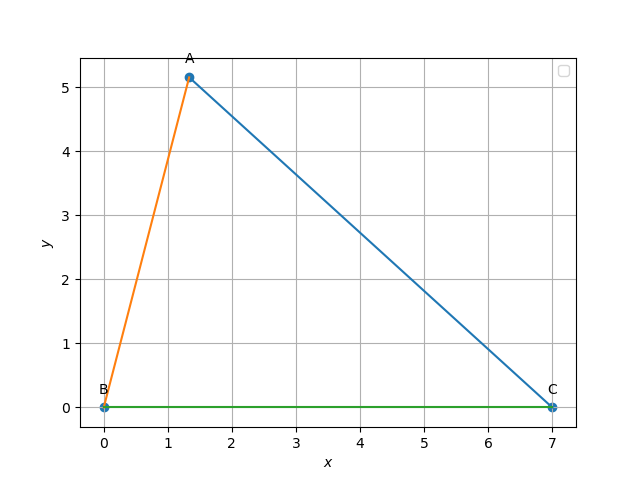
\includegraphics[width=\columnwidth]{chapters/9/11/2/1/figs/Figure_1.png}
		\caption{}
		\label{eq:cons/tri/9/11/2/1}
  	\end{figure}
	
	\vspace{3mm}
\section{Solution}
The input parameters for this construction are
\begin{center}
\begin{tabular}{|c|c|c|}
	\hline
	\textbf{Symbol}&\textbf{Value}&\textbf{Description}\\
	\hline
	BC & a & where a is 7cm\\
	\hline
	AB & b & AB distance is b \\
	\hline 
	AC & c & AC distance is c \\
	\hline
	$\angle{BC}$ & $75^0$ &  $\triangle$ABC \\
	\hline
	$\vec{C}$ & $\myvec{a\\0}$ & BC length is equal to a\\
	\hline
	$\vec{A}$ & $\myvec{ \cos\theta \\ \sin\theta}$ & using the cosine formula in $\triangle$ABC\\
	\hline
\end{tabular}
\end{center}
\raggedright {termux commands :}
\begin{center}
\fbox{\parbox{8.5cm}{bash line.sh.........using shell command}}
\end{center}
\raggedright\textbf{Caluclating Other Coordinate: } \\
\raggedright Let the coordinates of A are $X_{2}$,$Y_{2}$ respectively. \\
  \raggedright Let \textbf{A} =
  $\begin{pmatrix} 
 \cos \theta\\
  \sin\theta \\
\end{pmatrix}$ \\
\raggedright 
\fi
	Using the cosine formula in  $\triangle ABC$,
\begin{align}
	{b}^2&= {a}^2 + {c}^2 - 2ac\cos{B}
\\
\implies	(b+c)(b-c) &= {a}^2- 2  a  c\cos{B}
\\
	\text{or, }K(b-c) &= {a}^2- 2  a  c\cos{B}
		\label{eq:cons/tri/9/11/2/1/k}
\end{align}
%
where
\begin{align}
K = b+c 
		\label{eq:cons/tri/9/11/2/1/k/def}
\end{align}
From 
		\eqref{eq:cons/tri/9/11/2/1/k}
		and
		\eqref{eq:cons/tri/9/11/2/1/k/def},
\begin{align}
	\myvec{
		1 & 1
		\\
		1 & -1 
	}
	\myvec{
	b
	\\
	c
	}
	&=
	\myvec{
		\frac{{a}^2- 2  a  c\cos{B}}{K}
		\\
K}
\\
\implies
	\myvec{
	b
	\\
	c
	}
	&=
	\frac{1}{2}\myvec{
		1 & 1
		\\
		1 & -1 
	}
	\myvec{
		\frac{{a}^2- 2  a  c\cos{B}}{K}
	\\
K}
		\label{eq:cons/tri/9/11/2/1/k/mateq}
\\
\because
\myvec{
		1 & 1
		\\
		1 & -1 }
	\myvec{
		1 & 1
		\\
		1 & -1 }
	&	= 	{2}\vec{I}
\end{align}
From 
		\eqref{eq:cons/tri/9/11/2/1/k/mateq}
\begin{align}
	c
	&=
	\frac{1}{2}\vec{e}_2^{\top}\myvec{
		1 & 1
		\\
		1 & -1 
	}
	\myvec{
		\frac{{a}^2}{K}
	\\
	K}- \frac{2  a  c\cos{B}}{K}
\\
\implies
	c &=
	\frac{1}{2\brak{1+ \frac{2  a  \cos{B}}{K}}}\vec{e}_2^{\top}\myvec{
		1 & 1
		\\
		1 & -1 
	}
	\myvec{
		\frac{{a}^2}{K}
	\\
K}
\end{align}
The coordinates of $\triangle ABC$ can then be expressed as
\begin{align}
	\vec{A}=c\myvec{\cos B \\ \sin B},
	\vec{B} = \vec{0},
	\vec{C} =\myvec{a \\ 0}.
\end{align}
\iffalse
   reduced row echelon form of $\begin{pmatrix}13 & -13 + \frac{\sqrt{2} (-7 + 7 \sqrt{3})}{2} & 49\\1 & 1 & 13\end{pmatrix}$
        \vspace{3mm}
        \\Divide row1 by 13: R1 = $\frac{R1}{13}$
        \vspace{7mm}
 $        \begin{pmatrix} 1 & -\frac{ -7\sqrt{6}  + 7 \sqrt{2} + 26 )}{26} & \frac{49}{13}\\ 1& 1 & 13\end{pmatrix}$ \vspace{5mm}
        \\ Subtract row 1 from row 2: R2 = R2 - R1 \vspace{3mm}
        \\ $\begin{pmatrix}1 & -\frac{ -7\sqrt{6}  + 7 \sqrt{2} + 26 )}{26} & \frac{49}{13}\\ 0 & -\frac{ -7\sqrt{6}  + 7 \sqrt{2} + 52 )}{26} & \frac{120}{13}\end{pmatrix}$ \vspace{6mm}
         Multiply row 2 by $\frac{26}{- 7 \sqrt{6} + 7 \sqrt{2} + 52}$:\vspace{3mm}
         R2=$\frac{26}{- 7 \sqrt{6} + 7 \sqrt{2} + 52}$  
         \vspace{6mm}
    \\ Add row 2 multiplied by $\frac{- 7 \sqrt{6} + 7 \sqrt{2} + 26}{26}$ \vspace{5mm}
     \\  $\begin{pmatrix}1 & 0 &-\frac{ 91\sqrt{6}  + 91\sqrt{2} + 436)}{-7\sqrt{6}  + 7 \sqrt{2} + 52 )}\\ 0 & 1 &\frac{240}{ -7\sqrt{6} + 7 \sqrt{2} + 52} \end{pmatrix} $ \vspace{5mm}
     \\ $\begin{pmatrix}
     b \\
     c \\
     \end{pmatrix}$%
     = $\begin{pmatrix}
     -\frac{ 91\sqrt{6}  + 91\sqrt{2} + 436)}{-7\sqrt{6}  + 7 \sqrt{2} + 52 )} \\
     \frac{240}{ -7\sqrt{6} + 7 \sqrt{2} + 52}
     \end{pmatrix}$%
     \vspace{5mm}
    \\ \raggedright \textbf{A} = c$\begin{pmatrix}
                 \cos 75 \\ 
                 \sin 75 \\
              \end{pmatrix}$%
              =$\begin{pmatrix}
                 1.33 \\
                 5.15 \\
                 \end{pmatrix}$%
                 \vspace{5mm}
              \\ \raggedright  \textbf{B} = $\begin{pmatrix}
                 0\\
                 0\\
              \end{pmatrix}$% 
              \vspace{5mm}
             \\ \raggedright  \textbf{C} = $\begin{pmatrix}
                  7\\
                  0\\
              \end{pmatrix}$%
              \vspace{5mm}
\\
Below python code realizes the above construction : 
\fbox{\parbox{8.5cm}{\url{https://github.com/manasareddy442002/fwc-moudle1/blob/matrix-lines/matrix.py}}}

 \section{Construction}
 	\begin{center}
  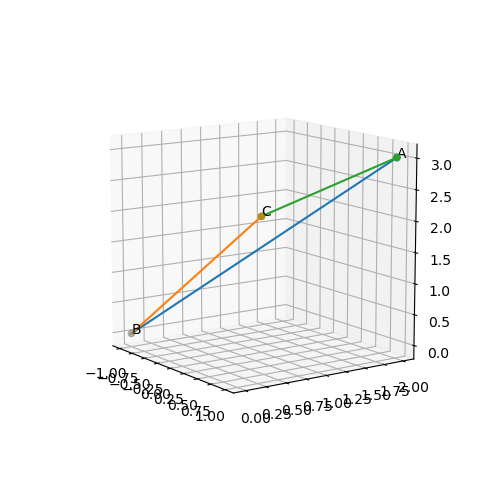
\includegraphics[scale=0.5]{Figure_1.png}
  	\end{center}
\vspace{3cm}
\end{multicols}

\end{document}
\fi
